\section{Introduction}

AGRAMMON is a model to simulate ammonia emission from farming. It
considers livestock (housing, yard, grazing), storage, application,
and plant production emissions of seven different animal categories
including 26 animal species. The most common housing systems for dairy
cows, cattle (tied and loose) and pigs (conventional ans label) are
considered as well as several different application
techniques. Ammonia emission of a single farm and of entire
Switzerland can be calculated. AGRAMMON has been developed by a group
of agronomists (SHL, Zollikofen), environmental scientists (Bonjour
Engineering GmbH, Lostorf) and computer scientists (Oetiker+Partner
AG, Olten) on behalf of the Federal Office for the Environment (FOEN,
Ittigen).

The Model is availabel for calculation under \texttt{http://www.agrammon.ch}.


\subsection{Structure of the model:}
The model consists of computing modules, technical parameters and input
parameters. 

\vspace{3ex}


\noindent The \textbf{input parameters} include terms such as animal
categories, number of animals, details on animal feeding, housing
system, storage, application, and plant production. These parameters
must be defined by the model users.

\vspace{3ex}

\noindent The \textbf{technical parameters} include terms such as
emission rates, emission factors, mobilisation- and immobilisation
rates of ammonia and ammonium, proportions of solid and liquid share
of the manure. Further information about animal feed like the
composition and the amount of the feed, the energy content, and the
crude protein content are defined in this section. The technical
parameters are assembled by the modellers considering the most recent
research results as well as international guidelines (e.g. UNECE 2007)
adopted for Switzerland. They can not be changed by the model users.

\vspace{3ex}

\noindent The process which calculates the ammonia emission by using
the input and the technical parameters is split into four main
computing modules: production (including excretion, housing, yard,
grazing), storage, application, and plant production (see Figure
1). Each module is divided into a number of submodules.


\vspace{12cm}
%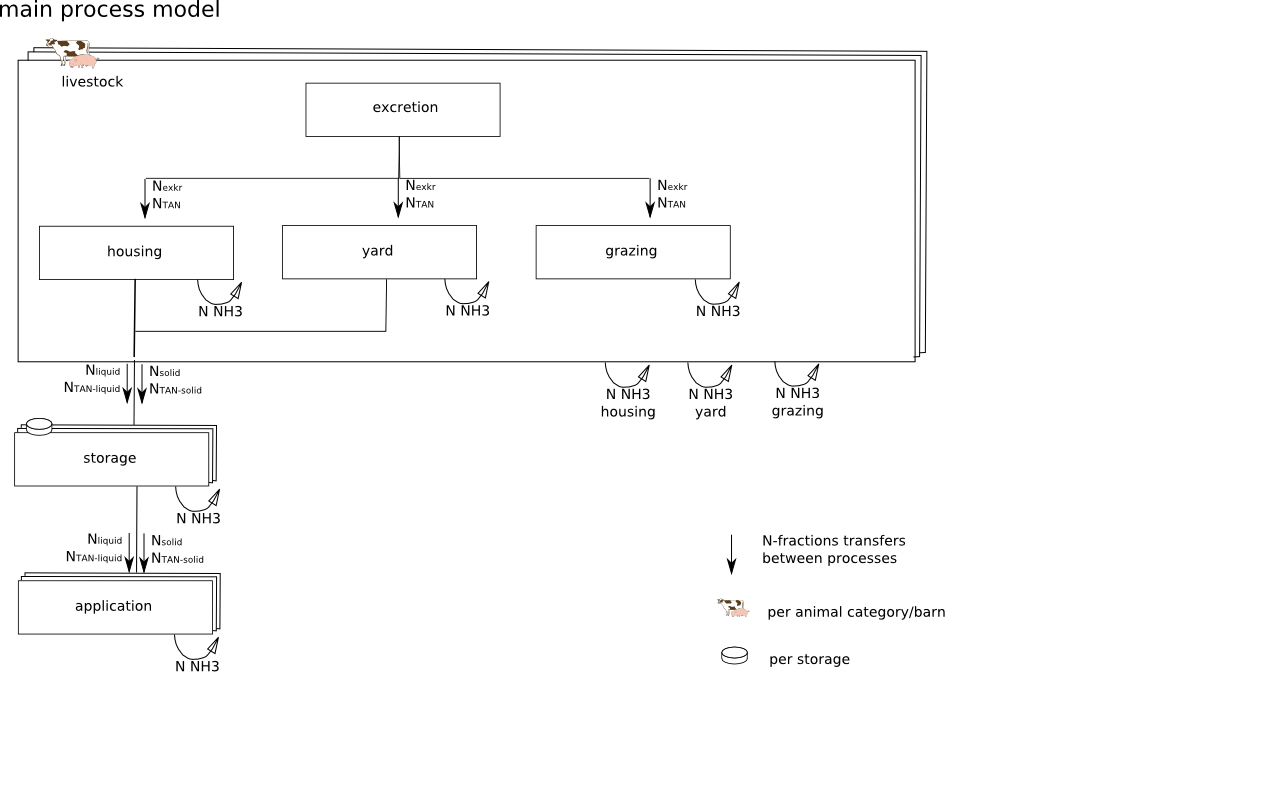
\includegraphics[width=160mm]{FluxSchemaWithoutFertil.png}
Figure 1: AGRAMMON process structure: livestock, storage, application, plant production

\subsection{Structure of the description:}

This technical process description shows the modules and submodules,
followed by the overall used input parameters and technical parameters
summarised in two tables at the end the document.

Modules and submodules are designed in a standardised manner with the
following sections: short description, input parameters, technical
parameters, output, detailed process description. The short
description gives a one line description of the module. Input
parameter, technical parameter and output are listed in tables
together with unit, value (tech. parameter), formula (output) and
description (input and tech. parameter). The detailed process
description gives additional information about the process including
references.




